\begin{savequote}[8cm]
The association of paternal and maternal chromosomes in pairs and their subsequent separation during the reducing division as indicated above may constitute the physical basis of the Mendelian law of heredity.
   \qauthor{--- \cite{Sutton1902morphology}}
\end{savequote}

\chapter{\label{ch:2-SDA} Single Cell Transcriptomics}

\minitoc

\section{Experimental Data Generation}

The experimental work in this chapter was performed by Min Jung and colleges in Don Conrad's group at the University of Washington, St Louis.

The samples generated are as follows:

\begin{itemize}
	\item 11 wild type C57BL/6 mice
	\item 3 FACS samples (primary spermatocyte , secondary spermatocyte, and spermatid) from a 12th wild type
%	\item 1 C57BL/6 mouse
	\item 1 sample of FACS sorted spermatogonial cells from 5 wild type C57BL/6 litter mates with GFP tagged Pou5f1 (B6;CBA-Tg(Pou5f1-EGFP)2Mnn/J, \cite{Szabo2002Allelespecific})
\end{itemize}

In addition to wild type mice four different mutant mice were included:
\begin{itemize}
	\item 6 \textit{Mlh3\textsuperscript{-/-}} mice (B6.129-Mlh3\textsuperscript{tm1Lpkn}/J, \cite{Lipkin2002Meiotic})
	\item 2 \textit{Hormad1\textsuperscript{-/-}} mice (B6;129S7-Hormad1\textsuperscript{tm1Rajk}/Mmjax, \cite{Shin2010Hormad1})
	\item 2 \textit{Cul4a\textsuperscript{-/-}} mice (B6;129-Cul4a\textsuperscript{-/-}, \cite{Yin2011E3})
	\item 2 CNP eGFP BAC TRAP (knockin) C57BL/6 mice (Joseph Dougherty).
\end{itemize}

The cells were dissociated by two methods: enzymatic for the first two wild type mice and the spermatogonia, and mechanical for all other samples \cite{Lima2017Standardized,Jung2019Unified}. The cells where then encapsulated using the DropSeq protocol \cite{Macosko2015Highly} as described in \cite{Jung2019Unified}.


\section{Data Processing and QC}

The samples were sequenced on either Illumina HiSeq2500 or MiSeq. Reads were mapped to the mouse using DropSeq tools provided by Macosko lab (using STAR aligner and GRCm38 release 90).

The resulting cell-gene count matrices were merged (54,251 cells and 38,317 genes) and processed through a series of quality control and normalization steps:

Genes with a UMI count of less than 5 or being expressed in fewer than 5 cells were removed.

Cells meeting the following criteria were removed:
\begin{itemize}
\item UMI count of less than 200
\item Fewer than 100 genes expressed
\item Log UMI count more than 1 standard deviation below the mean for that experiment
\item Log number of genes expressed was more than 1 standard deviation below the mean for that experiment
\end{itemize}

A tSNE dimensionality reduction of the filtered data revealed an amorphous homogeneous group of cells with low library size, high mitochondrial gene expression and often co-expressed genes from both early and late spermatogenesis suggesting poor quality and/or doublet cells. This group of cell was therefore removed before further analysis in addition to any cells with a normalised \textit{mt-Rnr-2} expression of greater than 2 suggestive of lysed cells \cite{Ilicic2016Classification}. These filters resulted in 20,322 cells and 28,893 genes remaining.

Genes in the lower third of expression means were then removed and cells were normalized by square root transformation of total transcript counts per cell and genes were normalized to unit variance. All expression values were capped to maximum of 10. This results in a final matrix of 20,322 cells by 19,262 genes with a sparsity of 93.8\% and a median UMI count of 1,312 per cell.


\section{SDA}

When performing a dimensionality reduction such as matrix factorisation we must somehow determine the number of latent components. Too low and we may miss some real components, too high and we may find spurious components due to overfitting. One way the method can overfit is by assigning a whole component to an individual cell, which we observed (Fig \ref{fig:single_cell_component}). We found when increasing the number of components from 50 to, 75, 100, 200 and 500 we got more of these single cell components rather than new normal components. With 50 components we had five individual cell components (1,4,8,14, and 46 - fig \ref{fig:SDA_diagnostics}) which we judged to be an acceptable balance between over and underfitting. We also ran SDA with five different random seeds to confirm stability of the results with different initialisations.


\begin{figure}[H]
	\centering
	\includegraphics[width=\textwidth]{figures/single_cell_component.pdf}
	\caption{Component 4 is represents a single cell.
		\textbf{(A)} Cell scores for component 4 ordered by value.
		\textbf{(B)} Gene loadings for component 4.
		\textbf{(C)} Predicted expression using only component 4 vs Raw Normalised Gene Expression. Pearson's correlation is quoted (equal to correlation with the gene loadings) . All of the genes with high expression in this cell have a high gene loading in this component.
		\textbf{(D)} As in C but for the cell with the second highest association. The correlation is much lower. 
		\textbf{(E)} As in C but using all components except 4. The correlation is less than C especially for highly expressed genes.
		\textbf{(F)} As in C but using all components for the prediction.  This is the sum of C and E
	}
	\label{fig:single_cell_component}
\end{figure}

By inspecting the change in free energy as well as the change in fraction of gene loadings with PIP < 0.5 we can confirm that the algorithm had converged within the 10,000 iterations for which it was run \ref{fig:SDA_diagnostics}. In addition the results are almost identical after 1,000 iterations (fig \ref{fig:10k}. Mean runtime for 10,000 iterations was 41.8 hours on a single core of Intel Xeon E5-2667 v4. The computational complexity of SDA scales with $NLC^2$ where N=number of cells, L=number of genes, and C=number of components. We acknowledge SDA is not the fastest way to analyse single cell RNA-seq data, however we prefer additional insight over gains in speed which for datasets of similar size to ours will be small relative to the time for data generation and analysis overall. As expected in line with previous reports from \cite{Hore2016Tensor} the PIPs have a bimodal distribution \ref{fig:SDA_diagnostics}.

\begin{figure}[H]
	\centering
	\includegraphics[width=\textwidth]{figures/SDA_diagnostics.pdf}
	\caption{Checking convergence of SDA.
		\textbf{(A)} Change in free energy is often 0 by the 10,000th iteration.
		\textbf{(B)} Change in fraction of PIP <0.5 is less than 0.005\%
		\textbf{(C)} Distribution of maximum scores and loadings for each component.
		\textbf{(D)} Distribution of PIPs across all components, showing expected bimodal distribution.}
	\label{fig:SDA_diagnostics}
\end{figure}

\begin{figure}[H]
	\centering
	\includegraphics[width=\textwidth]{figures/1k_vs_10k.pdf}
	\caption{Correlation of gene loadings between set inferrred using 1,000 iterations vs those using 10,000 iterations.}
	\label{fig:10k}
\end{figure}


The gene loadings are sparse with 79.8\% of the gene loadings having a PIP of less than 0.5 (fig \ref{fig:SDA}B,C). These genes have a tight distribution of loadings around 0 with a maximum absolute loading of 0.011 and 99\% of the loadings lying within the range (-0.0033, 0.0036). Of the gene loadings with a PIP of greater than 0.5 the maximum absolute loading is 1.31 and the mean is 0.062.


\section{Low Dimensional Visualisation}

\begin{figure}[H]
	\centering
	\includegraphics[width=\textwidth]{figures/tsne_random_seeds.png}
	\caption{
		\textbf{(A-C)} To quantify our uncertainty in the t-SNE embedding, we performed multiple t-SNE analyses with different random seeds. The cells are coloured by the same pseudotime values used throughout. Somatic cells are coloured gray. t-SNE coordinates are rotated about the origin to aid comparison.
		\textbf{(D)} We also performed dimensionality reduction using UMAP and confirmed that it gave a pseudotime embedding consistent with t-SNE. Cells are again coloured using the same psueodtime values as A-C}
	\label{fig:tSNEseeds}
\end{figure}

Despite reducing the dimensionality of the original dataset from 19,262 to 50 this is still too high to visualise the overall structure of the data. This can be achieved by performing a second non-linear reduction such as tSNE or UMAP (normally PCA is the linear reduction) \cite{Maaten2008Visualizing, McInnes2018UMAPa, Becht2018Dimensionality}. We find a horseshoe like effect often found when reducing datasets with an underlying 1 dimensional structure \cite{Novembre2008Interpreting, Podani2002RESEMBLANCE} (Fig \ref{fig:tSNEseeds}). By looking at genes with known expression patterns from the literature we can induce that in this case that the linear structure is developmental time of spermatogenesis and that the clusters in the centre are somatic cells (Fig \ref{fig:Marker_Genes}).


\begin{figure}[H]
	\centering
	\includegraphics[width=\textwidth]{figures/Marker_Genes.pdf}
	\caption{Imputed expression for genes with a range of expression patterns across cells}
	\label{fig:Marker_Genes}
\end{figure}

To generate a pseudo-timeline we used a similar approach to that implemented in SCUBA \cite{Marco2014Bifurcation}. We iteratively fit a principal curve through the t-SNE plot with increasing degrees of freedom from 4 to 9 using the curve from the previous run as the starting point \cite{Hastie1989Principal}. Each cell was then assigned to the closest position on this curve. Somatic cells and the Hormad1 X-activated cells (component 38 score >3) were excluded during pseudotime construction but the \textit{Hormad1\textsuperscript{-/-}} X-activated cells were given pseudotimes post-hoc. Somatic cells were defined by thresholding the cell scores of somatic components (if the absolute cell score of a given cell passed any of the following component thresholds 26, 11, 3, 32, 45, 24 > 2; 37 > 1.5; 40 > 1; or mt-Rnr2 expression >3).

The temporal order of components was determined by using a weighted mean of the pseudotime values, where the weights are the cell scores of the component. In addition, only those cells with an absolute cell score of greater than two contribute to the mean.

Although the model used for inference is symmetric for positive/negative gene weightings, many identified components showed strong biases towards positive or negative weights, consistent with expectations for identifying a group of co-activated (or co-repressed) genes (e.g. figure \ref{fig:SDA}E). Likewise, the cell loadings of each component frequently highlight specific cellular subsets that localize in t-SNE space and pseudotime (Figure \ref{fig:SDA} and \ref{fig:Cell_Scores})

\begin{figure}[H]
	\centering
	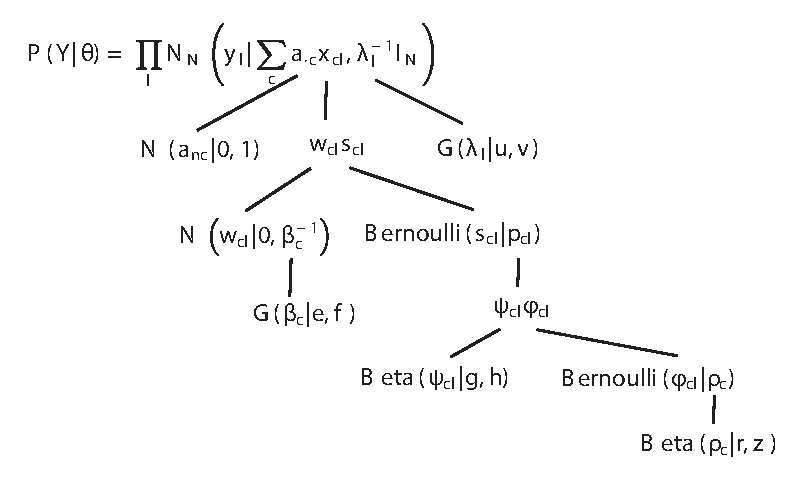
\includegraphics[width=\textwidth]{figures/SDA.pdf}
	\caption{
		\textbf{(A)} Schematic illustrating SDA
		\textbf{(B)} Density of gene loadings over all components with loadings separated into genes with PIPs > 0.5 (20\%) versus <0.5, indicating the sparsity of resulting gene loadings. PIP = Posterior Inclusion Probability that a gene loading is not equal to zero (i.e. not in the spike).
		\textbf{(C)} For each method, the fraction of all absolute gene loadings exceeding a ‘no loading’ sparsity threshold is shown, normalized by the maximum absolute loading across all components for that method. 
		\textbf{(D)} t-SNE projection of the cell scores from SDA. Each point it a cell, each coloured by their loading in component 5. Black arrow: the principle curve fit to the germ cell data, corresponding to the developmental ordering of each cell progressing through spermatogenesis. The coloured segmented line shows broad staging of spermatogenesis.
		\textbf{(E)} Gene loadings for component 5, plotted along the genome. Red genes: GWAS hits for human recombination rate.
		\textbf{(F)} Enrichment for GWAS hits of human recombination rate for all components. OR: Odds Ratio. P value by FET (main text). Positive (P) and negative (N) loadings are tested separately. For one-sided components (cell score range ratio >5) the minor side is omitted. Red horizontal line: p=0.05 after Bonferroni correction for multiple testing.
	}
	\label{fig:SDA}
\end{figure}

We can perform the same dimensionality reduction on the transposed cell scores or gene loadings to see how the components relate to each other (Fig \ref{fig:tSNE_Components}). We find 7 major clusters of components and with hindsight these correspond to: 1) Spermatogonia, 2) Leptotene/Zygotene 3) Pachytene 4) Round Spermatid (Acrosomal) 5) Spermiogenesis 6) Somatic and 7) Somatic (Sertoli). We can see that our manual labelling of the components is consistent with the clusters.

\begin{figure}[H]
	\centering
	\includegraphics[width=\textwidth]{figures/tSNE_Components.pdf}
	\caption{A low dimensional representation of the components shows 7 clusters.}
	\label{fig:tSNE_Components}
\end{figure}

Visualisation of components through pseudotime shows that transcription during spermatogenesis can be represented as a series of overlapping components, each varying with different timescales (Fig \ref{fig:SDA_overlapping} A\&B). Furthermore, these components are comprised of distinct gene sets enriched for distinct biological processes (Fig \ref{fig:SDA_overlapping} C\&D).

\begin{figure}[H]
	\centering
	\includegraphics[width=\textwidth]{figures/SDA_Overlaping.pdf}
	\caption{
		\textbf{(A)} For five example components, the cell scores for each cell are plotted through pseudotime, showing overlapping dynamic component activity. Component signs were chosen to be mainly positive (components have arbitrary sign). Color mappings as in panel B.
		\textbf{(B)} Stacked bar plot of cell component loadings for 14 germ components sorted by cell pseudotime. Each column corresponds to an individual cell and the total positive component loadings for each are normalized to one after flipping components to be mainly positive.
		\textbf{(C)} Shown are the top 10 gene loadings for each of the components in (B) represented as a heatmap. Most genes have strong loading on only one component.
		\textbf{(D)} Gene ontology enrichment analysis for biological processes in the top 250 genes for each component }
	\label{fig:SDA_overlapping}
\end{figure}



\section{Imputation}

In addition to identifying soft clusters and their marker genes, In the process of fitting the SDA model we have also effectively imputed the very sparse and noisy data. Multiplying out the cell scores and gene loadings matrix generates a matrix of the same dimensions as the original data but populated with the models predicted values. SDA imputation is able to estimate expression of individual genes even when in many cells zero reads are observed (Fig \ref{fig:imputation}A). In addition SDA expression estimates have fewer outlying high values outside the genes main expression window. The destructive nature of the single cell RNAseq protocol means that it is not possible to determine the true expression vector for an individual cell. In order to determine if imputation is actually improving our estimates we use cross-validation. Specifically, we randomly assign each read to either a training or test set, predict gene expression based on the training set (using SDA, or another method for example the dedicated imputation method MAGIC from \cite{vanDijk2018Recovering}) and then evaluate our ability to rank gene expression using the test set (methods). SDA imputation outperforms approaches using the raw data for essentially all cells in the test data (Fig \ref{fig:imputation}B\&C).

While providing the most sparse representation (Fig \label{fig:SDA}C), SDA still imputes equally well, compared to other matrix factorizations and MAGIC \parencite{vanDijk2018Recovering} (Fig \ref{fig:imputation}C \& \ref{fig:imputation_supp}A). Some cells gain more from imputation than others, the cells that gain the most are those with low library size (Fig \ref{fig:imputation_supp}C).

Furthermore, by comparing the genes with the lowest correlation between NNMF and SDA imputed expression, we found that SDA provides additional biological insights for the same number of components (Fig \ref{fig:imputation}D,E,F \& \ref{fig:imputation_supp}B). SDA infers multiple components for undifferentiated spermatogonia whereas NNMF only infers a single component resulting in imputed expression of \textit{Gfra1} and \textit{Lin28a} in the same cells (Fig \ref{fig:imputation}D and Figure \ref{fig:imputation_supp}B - no correlation for SDA component 50 \textit{Gfra1} Stem Cells). NNMF predicts a peak in the expression of X linked gene \textit{Rhox2h} even in WT cells, in which X chromosome activation due to Hormad1 KO does not occur suggesting underfitting of the data with 50 components (Fig \ref{fig:imputation}E). NNMF does not predict high expression of the adaptive immune cell marker \textit{Cd3g} (T-cell surface glycoprotein CD3 gamma chain), and when it predicts any expression it increases linearly with the innate immune cell marker \textit{Csf1r} (Macrophage Colony-Stimulating Factor 1 Receptor, or \textit{Cd115}) (Fig \ref{fig:imputation}F). In contrast SDA correctly predicts that \textit{Cd3g} and \textit{Csf1r} are not coexpressed in the same cells (See also \ref{fig:imputation_supp}B, no correlation for the SDA component 3 Lymphocytes).

In addition to obviating the need for further clustering and differential expression analyses, an advantage of using matrix factorization for imputation is the much smaller memory footprint required to store the results: on our dataset MAGIC data is 2.9 Gb whereas the SDA matrices are just 18 Mb (12.6 Mb when loadings with PIP <0.5 are set to 0).


\begin{figure}[H]
	\centering
	\includegraphics[width=\textwidth]{figures/imputation&NNMF.pdf}
	\caption{
		\textbf{(A)} For seven genes expressed at various stages of spermatogenesis unimputed normalised gene expression is shown alongside SDA imputed expression.
		\textbf{(B)} Prediction accuracy of seven predictors of gene expression trained on test data for an example individual cell. ‘Unimputed’ uses the training data directly, ‘Mean Cell’ uses the mean across all cells, matrix factorisation approaches SDA, PCA, ICA, NNMF, and a dedicated imputation approach, MAGIC.
		\textbf{(C)} Comparison of AUCs (Area under the curve) for all cells using various methods (same colour scheme as part B).
		\textbf{(D)} Zoomed versions of the t-SNE projection (with full t-SNE for context): cells are coloured by expression using a three channel ternary colour scheme with the amount of blue, green, red representing the respective expression levels of \textit{Lin28a}, \textit{Nanos1}, and \textit{Gfra1}.
		\textbf{(E)} Imputed expression of X chromosomal gene \textit{Rhox2h} from either the SDA or NNMF decomposition, split into cells we know to be either WT or \textit{Hormad1\textsuperscript{-/-}} genotype.
		\textbf{(F)} Imputed expression of \textit{Cd3g} and \textit{Csf1r} for both NNMF and SDA.}
	\label{fig:imputation}
\end{figure}

\begin{figure}[H]
	\centering
	\includegraphics[width=\textwidth]{figures/Imputation_Supp.pdf}
	\caption{
		\textbf{(A)} Imputed expression of an example gene (\textit{Smok2b}) for different methods, to illustrate the similar predictions as shown in Figure \ref{fig:imputation}B and \ref{fig:imputation}C.
		\textbf{(B)} Overall, NNMF infers similar components to SDA. The heatmap shows Pearson correlations between different pairs of gene loading vectors from SDA and NNMF (with procrustes rotation applied, Materials and methods).
		\textbf{(C)} The fold improvement in AUC when comparing SDA imputation to the unimputed data, plotted as a function of cell library size.
	}
	\label{fig:imputation_supp}
\end{figure}

\section{Mutant Genotypes}

Given we combined both wild-type and mutant cells in our analysis it is important to check that the components representing wild type processes are not unduly affected by this mixing. In order to quantify the robustness of our conclusions to this decision to combine mutant and wild-type strains, we performed a separate SDA analysis using just wild-type cells (the ‘WT’ analysis) and compared the results.

Factor analyses naturally have a degree of unidentifiability, whereas in SDA the sparsity prior helps to make the model identifiable across different seeds. For different data however the gene loadings matrix may be a rotated version in which components are linearly split or combined. A procrustean rotation can align two matrices (here gene loadings) onto an equivalent set of axes. Therefore, for fair comparison across SDA runs with different datasets, we compared the correlation of the gene loadings after procrustan rotation which tells us if the components inferred are effectively the same.

We found that most components generated from an SDA analysis of only wild-type data were also observed in the joint analysis of wild-type and mutant data. The most important WT components (those with high total cell score) have high correlations with components in the mixed SDA run (fig \ref{WT_vs_Mixed}). Some components such as Mix38 X activation are not represented in the WT decomposition because they represent mutant-specific processes. Other components such as Mix44 Leptotene-Zygotene do not appear as these cells are numerous only in mutant samples which lack the more abundant later stages of cells.

By visualising the rotation matrix from the procrustean analysis we can see which components have been rotated. For example Mix component 17 spermiogenesis is a linear combination of WT component 46 and 7 (fig \ref{fig:WT_Mix_Rotation}). We can also visualise the correlations directly as in figure \ref{fig:WT_Mix_Correlation}.

\begin{figure}[H]
	\centering
	\includegraphics[width=\textwidth]{figures/correlation_matrix_rotated.pdf}
	\caption{Here we show as a heatmap the pearson correlation of component gene loadings between a procrustean rotation of the WT gene loadings and the Mixed SDA gene loadings. The ‘sum abs cell score’ annotation shows the sum of the absolute cell scores for that component (larger number indicates a more important component). The ‘max cell score’ annotation indicates the maximum cell score for each component (a larger maximum indicates overfitting to a single/small number of cells).}
	\label{fig:WT_vs_Mixed}
\end{figure}

\begin{figure}[H]
	\centering
	\includegraphics[width=\textwidth]{figures/rotation_matrix_sparseNEW.pdf}
	\caption{This heatmap shows the procrustean rotation matrix (with absolute values < 0.35 rounded down to 0).}
	\label{fig:WT_Mix_Rotation}
\end{figure}

\begin{figure}[H]
	\centering
	\includegraphics[width=\textwidth]{figures/UdifSpg_gene_scatterplot.pdf}
	\caption{An example scatterplot comparing the gene loadings for one cognate SDA component (C31) between WT and Mixed SDA runs. The correlation is high.}
	\label{fig:WT_Mix_Correlation}
\end{figure}


\section{Non Meiotic Components}

Given we combined multiple experimental batches it's important to correct for batch effects and SDA provides a simple approach as some inferred components will capture these effects and can be removed.

Component 22 gene loadings are highly enriched in ribosomal proteins (50 of the top 100 loadings are non pseudogene ribosomal genes - of which there are 99, Fig \ref{fig:NonMeiotic}A). However unlike ribosomal component 43, the cell scores for component 22 are associated with whether the sequencing was done on MiSeq or HiSeq Illumina machines and so this component is likely a batch effect (Fig \ref{fig:NonMeiotic}B).

Component 12 has high cell loadings for \textit{Hormad1\textsuperscript{-/-}} cells, but these loadings are largely positive for the first two libraries, and negative for the last library (Fig \ref{fig:NonMeiotic}C,D).

Component 9 contains 41 out of 57 of the respiratory complex I, III, and IV genes (complex II is an alternative pathway) Fig \ref{fig:NonMeiotic}E,F (p = 7.4x10-53, OR = 104 [95\% CI: 62.1,Inf] FET). It's not clear whether this component reflects real meiotic biology or potentially reflects cell stress induced by experimental processing (still a real biological process but not one that exists in vivo).

\begin{figure}[H]
	\centering
	\includegraphics[width=\textwidth]{figures/NonMeiotic_Components.pdf}
	\caption{
		\textbf{(A \& B)} Gene loadings and cell scores for component 22.
		\textbf{(C and D)} Gene loadings and cell scores for component 12.
		\textbf{(E)} Gene loadings for component 9. Genes that are (non-assembly) components of the electron transport chain proton pump genes are highlighted in red. This gene set is defined by the genes that match the regex ‘Uqc|Cox|Ndu’. Pseudogenes, and genes with ‘assembly|like’ in their name were excluded.
		\textbf{(F)} Enrichment of genes that are (non-assembly) components of the electron transport chain proton pump genes in the top 500 genes from each component.
	}
	\label{fig:NonMeiotic}
\end{figure}


\section{Components}

Assigning a cytologically defined stage to each component requires considerable manual work due to lack of any high resolution data. There are a number of issues that complicate assignment. Firstly as we have seen components activities are gradual and so there may be no well defined set of cells or start and end to a component. Components can be mixed sign (positive/negative) and one sign may be active in a different stage to the other. Stages themselves are not well defined in the literature with multiple definitions being used by different groups. Due to translational regulation the transcription of genes may not correspond to the detection of the protein, hence using commonly performed antibody based immunofluorescence can be misleading and if available mRNA detection methods should be used for reference. In addition any literature references from human, or even rat, can have different expression patterns than mouse and so this evidence must be used with caution. Nonetheless using a combination of evidence types from multiple genes for each component we were able to assign almost all components to a stage(s) or cell type(s).


\begin{figure}[H]
	\centering
	\includegraphics[width=\textwidth]{figures/Cell_Scores.png}
	\caption{}
	\label{fig:Cell_Scores}
\end{figure}




\subsection{Telocytes}
Recently telocytes were discovered to be present in the mammalian (human) testis \parencite{Marini2018Reappraising, Kuroda2004Distribution}. We find one component (\#32) matching the known combination of markers for telocytes (\textit{Cd34} and \textit{Pdgfra} positive, \textit{Kit}, \textit{Pecam} and \textit{Acta2}/\textalpha-SMA negative) in addition to many other genes specific to this cluster (\textit{Dcn}, \textit{Col1a2}, \textit{Col1a2}, \textit{Col3a1}, \textit{Col6a1}, \textit{Col4a4}, \textit{Col4a1}, \textit{Col1a1}, \textit{Lamb1}, \textit{Lama2}, \textit{Lamb2}, \textit{Gsn}, \textit{Adamts5}, \textit{Mgp}) representing potential novel markers for this cell type in the testis. This component is highly enriched for the GO term "extracellular matrix organization" (p=4.3e-16, OR=10.3). Their expression pattern matches what was described as an unknown mesenchymal cell population by \cite{Green2018Comprehensive} with expression of \textit{Tcf21}, \textit{Arx}, \textit{Vim}, and \textit{Col1A1}, but not \textit{Acta2} (\textalpha-SMA), or \textit{Cyp17a1}.


\subsection{Leydig Cells}
Component 40 broadly marks all Leydig cells and has high gene loadings for all the major genes required for testosterone production including \textit{Star}, \textit{Cyp11a1}, \textit{Hsd3b}, \textit{Cyp17a1}, and \textit{Hsd17b} \ref{fig:testoterone} \cite{Stojkov2013Orally} in addition to other markers of Leydig cells including \textit{Insl3} and \textit{Ptgds} \parencite{Balvers1998RelaxinLike, Baker2001Expression}. This component is most highly enriched for the GO term "steroid metabolic process" (p=5.3e-23, OR=11.3)

Component 26 splits Leydig cells into two main groups, distinguished by the expression of \textit{Fabp3}, \textit{Gstm1}, \textit{Gsta3}, and \textit{Ass1}.

Component 24 is a subtype of the \textit{Fabp3} expressing C26 positive cells, which has high expression of \textit{Gstm3}, \textit{Mt3}, \textit{Thrsp}, and \textit{Jak3}, but also a number of pseudogene versions of genes that are normally expressed leydig genes: \textit{Gstm2-ps1}, \textit{Gm6665} (another \textit{Gstm2} pseudogene), \textit{Fabp3-ps1}, \textit{Gm8834} (\textit{Gstm3} pseudogene), \textit{Gm5096} (\textit{Bhmt} pseudogene), \textit{Gm6977} (\textit{Fth1} pseudogene), \textit{Gm7049} (\textit{Me1} pseudogene).

Component 19 marks cells in both major groups and is distinguished by high expression of a group endopeptidases encoded in a 300kb locus on chromosome 7 including \textit{Klk1}, \textit{Klk1b1}, \textit{Klk1b21}, \textit{Klk1b22}, \textit{Klk1b24} and \textit{Klk1b27}. Some of these genes are known to be specifically expressed in Leydig cells and may be involved in remodelling of the extracellular matrix \parencite{Sanz2013RiboTag, Matsui2000Cloning, Matsui2001Mouse, Matsui2005Characterization}.

\subsection{Sertoli Cells}

Component 37 is active in cells expressing \textit{Wipf3} (aka CR16) and \textit{Ncoa2} (aka TIF2) both of which are required for fertility and have Sertoli restricted expression \cite{Suetsugu2007Malespecific, Gehin2002Function}). In addition \textit{Nxf3} is specifically expressed in Sertoli cells but not required for spermatogenesis \cite{Zhou2011Nxf3}.

%45

%16

\subsection{Macrophages}
We find one component (\#11) representing macrophage cells. This component has high loadings for \textit{Csf1r} (macrophage colony-stimulating factor receptor, aka CD115), \textit{Cd163} (macrophage scavenger receptor), \textit{Cd68}, \textit{Adgre1} (aka F4/80), \textit{Itgam} (aka CD11b), \textit{Mrc1}, \textit{Cx3cr1}, \textit{Fcgr3}, and the complement genes \textit{C1qa}, \textit{C1qb}, and \textit{C1qc}. \parencite{Mossadegh-Keller2017Developmental, Fabriek2005macrophage, Sasmono2012Generation}

Immunohistochemical staining of ADGRE1 found that macrophages were present within the tubule, which is typically regarded as immune privileged partly due to the blood-testis barrier formed by sertoli cell tight junctions \parencite{Fijak2006testis}. Macrophages have previously been reported within the adluminal compartment, although always in the context of testicular defects \parencite{Frungieri2002Number, Goluza2014Macrophages}.


\subsection{Lymphocytes}
Component 3 is highly enriched for genes involved in T cell activation (p=1.4e-19, OR=7.6) and has high loadings for (T-cell) lyphocyte genes including \textit{Ptprc} (aka CD45, leukocyte common antigen), \textit{Cd2} (aka T-cell surface antigen) \parencite{Murray2011Protective, Murphy2012Janeway}, \textit{Ms4a4b} (high protein expression in T and NK but not B cells \cite{Xu2010MS4a4B}), and the CD3 T-cell receptor complex genes: \textit{Cd3g}, \textit{Cd3d}, \textit{Cd3e}, \textit{Trbc2}, \textit{Trac} \parencite{Call2002Organizing}.


\subsection{Peritubular Myoid}
% 21??

Component 10 is active in a small number of cells, likely to be peritubular myoid cells due to co-expression of \textit{Cnn3}, \textit{Edn1} (Endothelin), \textit{Myh11} (Smooth muscle myosin heavy chain), and \textit{Acta2} (Smooth muscle actin) \parencite{Mayerhofer2013Human}. The most significant GO term is "muscle tissue development" (p=8.789135e-08, OR=4.97).





\subsection{Spermatogonia}

% Spermatogonia can are the most undifferentiated germ cells in the adult body. There are a number of different types which can be categorised according to the Oakberg scheme in mice \parencite{Oakberg1971Spermatogonial}. As are the most stem cell like, which divide into Apr, Aal4, Aal be \parencite{vanPelt1990Synchronization}

Five components correspond to processes in spermatogonia. Component 31 represents undifferentiated spermatogonia expressing \textit{Zbtb16} (aka \textit{Plzf}) \parencite{Buaas2004Plzf} and \textit{Foxo1} \parencite{Goertz2011Foxo1}, while component 50 splits these into two subpopulations one expressing, \textit{Gfra1} (shown to be expressed in a subset of As and required for As self renewal by acting as a co-receptor for GNDF \parencite{Meng2000Regulation,He2007Gfra1}) and \textit{Glis3} \parencite{Kang2016Transcription}, and the other \textit{Nanos3} \parencite{Suzuki2009heterogeneity}, \textit{Lin28a} \parencite{Zheng2009pluripotency} and \textit{Foxf1}. Component 7 likely represents A1-4 spermatogonia as they express c-Kit which is expressed in differentiated (not undifferentiated) spermatogonia \parencite{Manova1990Gonadal,Schrans-Stassen1999Differential} and is required for the A1 to Al divisions \parencite{Yoshinaga1991Role}. These cells also express \textit{Stra8} which is expressed from type A spermatogonia through to preleptotene cells in response to retinoic acid \parencite{Oulad-Abdelghani1996Characterization,Zhou2008Expressiona,Endo2015Periodic} and is required for premeiotic DNA replication \parencite{Baltus2006germ}. We find they these cells are also well marked by \textit{Plppr3}, \textit{Sertad4}, \textit{Met}, \textit{Jade2}, \textit{Nanos1}, \textit{Glis1} and \textit{Glis2}. Component 2 includes \textit{Ctcfl}, \textit{Pou4f1}, and \textit{Esx1} - likely representing intermediate and type B spermatogonia \parencite{Sleutels2012male, Budhram-Mahadeo2001closely, Maezawa2018Dynamic, Li1997Esx1, Branford1997Spx1}. Component 33 is broad component covering all the stages of spermatogonia.


\subsection{(pre)Leptotene \& Zygotene}

Component 5 includes many genes required for the creation and repair of meiotic double strand breaks. This includes \textit{Prdm9} itself; components of the meiotic cohesin complex \textit{Rad21l}, \textit{Smc1b}, \textit{Smc3}, \textit{Stag3} and \textit{Esco2} \parencite{Rankin2015Complex}; components of the telomere tethering complex \textit{Terb1}, \textit{Terb2}, \textit{Spdya}, and \textit{Sun1} \parencite{Ding2007SUN1, Tu2017Speedy, Wang2019meiotic}; genes involved in creating DSBs \textit{Mei1}, \textit{Ccdc36} (\textit{Iho1}), \textit{Spo11} partner \textit{Top6bl} (\textit{Gm960}), and regulator \textit{Atm} \parencite{Lukaszewicz2018Control, Reinholdt2005Mei1, Robert2016TopoVIBLike, Stanzione2016Meiotic, Vrielynck2016DNA}; proteins required for the creation and processing of the ssDNA intermediates and their regulators: \textit{Mcm8}, \textit{Dmc1}, \textit{Rad51}, \textit{Rad51ap2}, \textit{Atr}, \textit{Brca2}, \textit{Tex15}, \textit{Meilb2} (\textit{Hsf2bp}), \textit{Meiob}, and \textit{Spata22} \parencite{Brown2015Small, Brown2014DNA, Dai2017Meiotic, Kovalenko2006RAD51AP2, Lee2015MCM89, Martinez2016BRCA2, Pacheco2018ATR, Ribeiro2018MEIOB, Widger2018ATR, Xu2017Meiosisspecific, Yang2008Mouse, Zhang2019meiosisspecific}; class I crossover (ZMM group) proteins \textit{Shoc1} (\textit{Zip2} orthologue), \textit{Tex11} (\textit{Zip4} orthologue), \textit{Msh5}, \textit{Hfm1} (\textit{Mer3} orthologue) and regulator \textit{Brip1} (\textit{FancJ}) \parencite{Adelman2008ZIP4H, Guiraldelli2018SHOC1, Guiraldelli2013Mouse, Rakshambikai2013Structural, Sun2016FancJ}; as well as components of the synaptonemal complex \textit{Sycp1}, \textit{Sycp2}, \textit{Sycp3}, \textit{Syce2}, \textit{Syce3}, \textit{Tex12}, and \textit{Six6os1} (\textit{4930447C04Rik}) \parencite{Gomez-H2016C14ORF39, Syrjanen2014molecular}.


This component is also highly enriched for GWAS hits of recombination rate in Icelandic humans \cite{Halldorsson2019Characterizing}. Of the 24 significant GWAS loci identified with confidently associated causal genes, more than half (13) rank within the top 300 genes of this component, and almost all (20) rank within the top 1300 genes (p = 5.2x10-18, OR = 77.8 [95\% CI:36.4,Inf] and p = 2.4x10-20, OR = 70.1 [95\% CI:26.9,Inf]] respectively by fisher's exact test [FET]). One of the hits, \textit{Msh4}, is not ranked highly in this component (2734th out of 19262), however, it is known to function as a heterodimer with \textit{Msh5}, which ranks 34th \cite{Rakshambikai2013Structural}. This highlights one of the advantages of single cell RNAseq compared to GWAS for target discovery in that it does not rely on the presence of (perhaps rare, small effect) genetic variants. In addition it directly provides a list of genes rather than SNPs affecting unknown causal genes, For example the previous GWAS had identified a SNP in the intron of \textit{Ccdc43}, however our expression data strongly suggested the adjacent gene \textit{Meioc} (aka \textit{C17orf104}) as the causal gene (ranked 183rd vs 13,651st in component 5) in addition to the subsequent reports that \textit{Meioc} is responsible for maintaining an extended meiotic prophase \cite{Abby2016Implementation, Kong2014Common, Soh2017Meioc}. 

The strong enrichment of genes involved in recombination in this component suggests other highly ranked genes of unknown function could also play key roles in this process. This proved to be the case for two such genes during the preparation of this manuscript. Firstly \textit{Ankrd31} (ranked 102nd) was found to control the number, timing, and location of double strand breaks in meiosis \cite{Boekhout2018REC114, Papanikos2018ANKRD31} and \textit{Hsf2bp} (now \textit{Meilb2}, ranked 194th) was found to be a master regulator of meiotic recombinases \cite{Zhang2019meiosisspecific}. One candidate, \textit{Zcwpw1}, will be the subject of the second part of this thesis.


\subsection{Pachytene}

Testis specific lactate dehydrogenase \textit{Ldhc} \parencite{Goldberg1963Lactic, Blanco1963Lactate, Goldberg2010LDHC}, in addition to \textit{Ldha} and \textit{Ldhal6b} \parencite{Wang2005Cloning}, and another glycolytic enzyme \textit{Pgam2} for which protein expression was found from pachytene onwards \parencite{Fundele1987Developmental}.

Y-box proteins are abundant in spermatocytes where they bind to and repress translation of mRNA \parencite[Reviwed in]{Kleene2016Positiondependent}. \textit{Ybx2} (aka \textit{Mys2}) which was found translated from pachytene onwards \parencite{Kwon1993Proteins, Oko1996Germ} (transcribed from day 17 \& in pachytene cells \parencite{Gu1998Mammalian}) and is required for fertility \parencite{Yang2005Absence}. \textit{Ybx1} (\textit{Msy1}) also has a high loading, with reported mRNA detectable by northern blot from day 15 (pachytene) \parencite{Tafuri1993mouse}. \textit{Ybx3} (aka \textit{Msy4}), has a high loading and is detected as protein in mid-pachytene cells \parencite{Davies2000SequenceSpecific}] and extended expression causes infertility \parencite{Giorgini2002Translational}

Poly(A) binding proteins also bind to and regulate mRNA \parencite[reviewed in]{OZTURK2018Potential}. \textit{Pabpc1} and \textit{Pabpc2} both have high loadings in component 42 and are detectable from pachytene onwards \parencite{C.Kleene1994Developmental, Gu1995Poly, Kleene1998Mouse, Lee2000Expression, Kimura2009Characterization}. \textit{Pabpc6} also has a high loading but is understudied in comparison.

Pachytene components can be readily identified by the relative lack of loadings on the X and Y chromosomes \ref{fig:MSCI}D,E. This is due to a process whereby when homologous partners fail to synapse they are marked by HORMAD1, HORMAD2 and BRCA1. This is followed by recruitment of ATR and the creation of $\gamma$H2AX resulting in transcriptional silencing (Meiotic Silencing of Unsynapsed Chromatin). As the X and Y chromosomes are only partially homologous they fail to fully synapse and are silenced by this processes (Meiotic Sex Chromosome Inactivation, MSCI) \parencite{Turner2007Meiotic, Turner2015Meiotic}.

Pseudotime analysis provides quantitative, high-resolution insights into meiotic sex chromosome inactivation (MSCI). We are able to track this process through pseudotime by visualising the ratio of sex to autosomal expression through pseudotime (Fig \ref{fig:MSCI}A \& \ref{fig:MSCI_supp}A). The ratio drops sharply (possibly exaggerated by inefficient cell capture) to close to 0 before gradually recovering, although to a level below that of the original starting ratio. It has previously been reported that some sex chromosome genes are able to escape MSCI \parencite{daCruz2016Transcriptome, Soumillon2013Cellular}. However, we were unable to detect expression of these genes during the time at which MSCI is active (Fig \ref{fig:MSCI}C \& \ref{fig:MSCI_supp}B). Many of the genes had high expression just before or after MSCI, suggesting that they were previously identified due to the low stage-resolution of the previous study. 

\begin{figure}[H]
	\centering
	\includegraphics[width=\textwidth]{figures/MSCI.pdf}
	\caption{
		\textbf{(A)} The sum of imputed expression for all genes on the X chromosome divided by that of the autosomes (y-axis).
		\textbf{(B)} We do not observe that haploid cells obviously split into two populations due to lack of sex chromosome transcript sharing, in part A. Here were simulate what we might expect to see if there was indeed a lack of sharing (Materials and methods).
		\textbf{(C)} Smoothed expression values (unimputed, adaptive GAM smoothing with formula ‘y ~ s(x, bs = ad)") are shown for each gene reported to escape MSCI \parencite{daCruz2016Transcriptome} excepting \textit{H2al1e}, \textit{H2al1c}, and \textit{Gm10096} which were below our dataset's expression detection threshold.
		\textbf{(D)} Component 42 (Pachytene) cell scores in t-SNE space.
		\textbf{(E)} Component 42 gene loadings. This component represents genes active during the pachytene stage of meiosis; note the striking lack of sex chromosome gene loadings, due to MSCI.
	}
	\label{fig:MSCI}
\end{figure}

\begin{figure}[H]
	\centering
	\includegraphics[width=\textwidth]{figures/MSCI_supp.pdf}
	\caption{
		\textbf{(A)} As for Figure \ref{fig:MSCI}A, but Y chromosome instead of X. Due to lower number of expressed genes on the Y chromosome MSCI is not as clear and individual genes can influence the overall ratio to a large degree.
		\textbf{(B)} As for Figure \ref{fig:MSCI}C, but each gene is shown individually.}
	\label{fig:MSCI_supp}
\end{figure}


In addition to MSCI we may expect to observe a lack of sex chromosome transcripts due to the lack of either an X or Y chromosome in the haploid cells post meiotic division. However, from the mitotic divisions of the spermatogonia onwards cytokinesis does not fully complete and $um$-wide cytoplasmic bridges are formed between adjacent cells such that the cytoplasm could be shared across a synctium of cells \cite{Greenbaum2011Germ}. Whilst theoretically thousands of cells could be connected in practise up to 650 connected cells have been observed \cite{Ren1991Clonal}. The extent to which mRNA sharing occurs is unknown although efficient sharing has been shown for individual genes \cite{Braun1989Genetically}. If many genes were not shared we would expect to see two populations of cells after the meiotic divisions with high and low X chromosome expression respectively. However, we observe a marginal distribution of X expression conditional on pseudotime that is unimodal - suggesting that mRNA (on the X chromosome at least) is efficiently shared (Fig \ref{fig:MSCI}B).

There remains a possibility that some individual or group of genes are not shared, such as has been observed for autosomal genes in a mutant heterozygous context: the t-complex responder mutant (\textit{SmokTcr}) which functions as an antidote in the poison-antidote meiotic drive system of the t-complex \cite{Veron2009Retention} and \textit{Spam1} which causes transmission ratio distortion in Robertsonian (Rb) translocation-bearing mice \cite{Martin-DeLeon2005Spam1associated}.

\subsection{Hormad1 Sex Chromosome Activation}
In addition to the pachytene components with lack of loadings on the sex chromosome we also find a component (\#39) with an \textit{excess} of sex chromosome loadings relative to the autosomes (fig \ref{fig:Hormad1}A). This component is active exclusively in a subset of Hormad1 KO cells that diverge from the normal pseudotime around Zygotene stage \label{fig:MiscComponents}C. Note that as Hormad1 KO mice arrest at early Pachytene, once the cells diverge the pseudotimes can no longer be compared to the wild type pachytene cells and are perhaps considerably compressed due to the almost perpendicular direction \parencite{Shin2010Hormad1}. HORMAD1 marks unsynapsed chromosomes, so when HORAMD1 is absent (as in the KO) it appears as though the sex chromosomes are fully synapsed and transcriptional silencing fails to occur. We find that not only does Hormad1 KO fail to silence previously expressed sex-linked genes, many previously \textit{unexpressed} sex-linked genes such as Rhox2h have high expression (fig \ref{fig:Hormad1}B). Interestingly, there are also multiple autosomal genes with high loadings. This may be due to ectopic expression of sex-linked transcription factors; for example, \textit{Zfy1} and \textit{Zfy2} were previously shown to cause pachytene arrest when forcibly expressed \cite{Royo2010Evidence}. We find a very strong association between genes in this component and genes overexpressed in mice which have mutations in either \textit{Hormad1} ($p = 2.2x10^{-39}$ OR = 184) or \textit{Trip13} which is required for HORMAD1 removal from synapsed chromosomes ($p = 1.3x10^{-157}$ OR = 115) \cite{Ortega2016Surveillance, Wojtasz2009Mouse} (fig \label{fig:MiscComponents}A,B).

\begin{figure}[H]
	\centering
	\includegraphics[width=\textwidth]{figures/Hormad1_two.pdf}
	\caption{
		\textbf{(A)} Gene loadings for component \#39 shown along the genome.
		\textbf{(B)} Gene expression for high loadings genes from chromosome 1 (\textit{A830018L16Rik}) and X (\textit{Rhox2h}).
	}
	\label{fig:Hormad1}
\end{figure}

\subsection{Meiotic Divisions}
Component 20 contains high loadings for cell cycle associated genes such as the cyclin \textit{Ccna1} which is expressed from late pachytene through until just after the meiotic divisions \parencite{Sweeney1996distinct} for which it is required \parencite{Liu1998Cyclin}. The cyclin \textit{Ccnb1} controlling the G2/M transition is also present, along with its activators \textit{Aurka}, \textit{Bora}, \textit{Plk1}, and \textit{Cdc25a} \parencite[Reviewed in ]{Joukov2018AuroraPLK1}. The CDK2 inhibitor \textit{Cdkn3} (aka KAP1, \parencite{Poon1995Dephosphorylation}), \textit{Rgcc} (regulator of cell cyle) which is required for G2/M transition \parencite{Saigusa2007RGC32}, anaphase promoting complex activator and \textit{Cdc20} homologue \textit{Fzr1} \parencite{Holt2014APC}, and Mitotic Checkpoint Complex antagonist \textit{Mad2l1bp} (\textit{p31comet}) \parencite{Habu2002Identification}.

The positive and negative loadings are marginally significantly enriched for ``spindle checkpoint'' and ``chromosome segregation'' GO terms respectively (p= 0.03 \& 0.015, OR= 10.4 \& 3.7).

This component is also highly enriched for a family of proteins with a domain of unknown function (DUF622) \textit{1700001F09Rik}, \textit{Gm3453}, \textit{Gm10354}, \textit{Gm3149}, \textit{Gm8362}, \textit{Gm3127}, \textit{Gm17019}, \textit{Gm4181}, \textit{Speer4e}, \textit{Speer4b}, \textit{Gm9758}, \textit{Gm8232}, \textit{BC061237}, \textit{Gm5458}, \textit{4930572O03Rik}, \textit{Gm5800}, \textit{Gm7361}, \textit{Gm8220} (18 out of the top 88 genes). This family of genes is rodent specific and arose from duplication of the \textit{Dlg5} gene \parencite{Church2009Lineagespecific}. Interestingly it was reported that genes of this family have similar epigenetic profiles to that of the sex chromosomes in spermatogenesis \parencite{Moretti2016Expression}. This component is also host to a second family of ampliconic genes (Ssx - Synovial Sarcoma associated, on the X chromosome), discussed in further detail below.

\subsection{Round Spermatid}
Round spermatid component 30 contains many genes associated with the acrosome, an organelle which forms a nuclear cap containing hydrolytic enzymes used in fertilization (Ito and Toshimori, 2016) (Supplementary file 3). For one high loading gene, \textit{Lrrc34}, we verified by immunofluorescence that the protein is indeed localized to the acrosome of round spermatids (Figure 2B). Component 35, which is essentially concurrent to component 30 in pseudotime, is the most mysterious of all components that we detected. Dozens of protein-coding genes in this component are highly enriched in testis expression but have no known function (Supplementary file 3). This component also harbors a substantial number of genes with no apparent ortholog in humans. The existence of such a set of poorly characterized genes likely reflects the difficulty of studying postmeiotic male germ cells - which cannot be differentiated in vitro, host numerous cell-type specific processes, and express many rapidly evolving genes.

\subsection{Spermatocytes}

The spermiogenesis components 17, 18 and 34 all contain many genes known to be expressed at the latest stages of spermatogenesis, before transcriptional arrest due to replacement of histones with protamines (Sassone-Corsi, 2002) (Supplementary file 3). In addition, \textit{Abhd5} (aka CGI-58), a protein previously detected in testis lipid droplets (Wang et al., 2015), has high loadings specifically in these late components (17 and 18) and we show by immunofluorescence that it serves as an excellent marker of the residual body (Figure 2B).


\begin{figure}[H]
	\centering
	\includegraphics[width=\textwidth]{figures/Fig4_S3.pdf}
	\caption{
		\textbf{(A)} Enrichment of component 38 gene loadings for genes previously identified as overexpressed in both \textit{Trip13\textsuperscript{-/-}} and \textit{Hormad1\textsuperscript{-/-}} mutants. Component 38 (X Activation) gene loadings are shown ordered by rank (high-to-low) with the genes previously identified as overexpressed in \textit{Hormad1\textsuperscript{-/-}} and \textit{Trip13\textsuperscript{-/-}} mice highlighted as rug plots.
		\textbf{(B)} Fisher’s test was used to test for enrichment of genes previously identified as overexpressed in \textit{Hormad1\textsuperscript{-/-}} and \textit{Trip13\textsuperscript{-/-}} mice in the top 500 genes of each component. Positive and negative loadings for each component are analyzed separately; thus 38N is the negative gene loadings for component 38 and 38P the positive ones. The positive loadings of component 38 are highly and specifically enriched for these genes. Component enrichments are further colored red and blue to indicate the primary cell type with loading on each component (red = germ cell, blue = somatic cell). 
		\textbf{(C)} Cell scores for component 38 in t-SNE space. The cells with component 38 active are localized to a group of cells which diverge from the pseudotime-line just before pachytene.
		\textbf{(D)} MSCI in t-SNE space. The cells with active component 38 also have a high ratio of sex to autosome expression ratio, showing that not only do these cells fail to silence sex linked genes but they are actively overexpressed.
		\textbf{(E)} Gene loadings and cell scores for component 11 (Macrophages). Genes with GWAS signals for Alzheimers disease are highlighted in red. (F) Gene loadings for component 40 (Leydig cells), with key genes of testosterone synthesis highlighted in red. The pathway of testosterone synthesis is shown with genes that have high loadings in component 40 highlighted (Adapted from Stojkov et al., 2013).
	}
	\label{fig:MiscComponents}
\end{figure}


\section{Motif Inference}
Given there exists these groups of co-expressed genes the obvious question is what's driving this expression? One major class of transcriptional regulation is the binding of transcription factors to promoters and enhancers.

\subsection{Enrichment of Known Transcription Factor Targets}
There are some transcription factors that are known to regulate meiotic gene expression. One of these is MYBA (encoded by \textit{Mybl1}, \cite{Bolcun-Filas2011AMYB}) and we find that the predicted direct targets of the MYBA transcription factor ()as found by ChIPseq and RNAseq of KO mice) are strongly enriched specifically in the pachytene components as expected based on known targets and expression of \textit{Mybl1}. Other known meiotic transcription factors including \textit{Stra8} \parencite{Kojima2019Amplification}, \textit{Rfx2} \parencite{Kistler2015RFX2}, and \textit{Crem} \parencite{Nantel1996Spermiogenesis} are also enriched in specific components contiguous in pseudotime and consistent with their known targets.


\subsection{\emph{De-novo} inference form promoter sequences}
Transcription factors are able to recognise specific subsets of gene promoters by sequence specific binding to DNA motifs. Hence, if transcription factors are responsible for the co-expression patterns observed, we would expect to see enrichment of these binding motifs in the promoters of the co-expressed genes. However, it is possible that there are undiscovered transcription factors and or binding motifs and so instead we inferred \textit{de novo} motifs from the promoter sequences of the top genes from each component. This resulted in 16 groups of motifs including matches to the master regulators \textit{Stra8}, \textit{Mybl1}, \textit{Rfx2}, \textit{Crem}, as well as other genes required for fertility \textit{Nrf1}, \textit{Etv5}, \textit{Zfp143}, and \textit{Rara}.

\subsection{Broad-scale patterns of TFBS occurrence over PseudoTime}
Many motifs were found from multiple components and so to gain a broader view of which components these motifs act in we computed the linear association between the gene loadings and the motif presence probability for each motif-component combination. The known master regulators showed relatively specific enrichment (e.g. \textit{Stra8} in Leptotene component \#5, \textit{Mybl1} in Pachytene component \#42, and \textit{Rfx2} in Acrosomal component \#30). Most motifs, however, have a broad pattern of enrichment in either the diploid components or the haploid components. Other mechanisms which could control the fine-scale patterns of transcription we observe are transcription factor binding at enhancers (in which we did not look for motifs given their unknown locations and gene associations), chromatin status (modulating transcription factor binding), and or differential mRNA degradation.

We discovered that many of the motifs which show similar associations through pseudotime share a common property: the presence of a CpG dinucleotide. Many of diploid motifs contain a CpG dinucleotide whereas most of the haploid motifs do not. In fact the motif with the strongest association with pseudotime is not a motif per-se but simply the count of CpGs at the promoter.

CpG islands at active promoters are usually unmethylated and methylation can cause silencing \parencite{Li2014DNA}. 

Many of the diploid CpG containing motifs have methylation sensitive transcription factors, including the non-CpG exceptions NFYA and ETV5 \parencite{Domcke2015Competition, Wang2017NRF1}. This suggests that methylation may play a role in the mechanism by which the type of transcription factor used pre and post division is switched.

There are many genes that are expressed around the time of the meiotic divisions in component 20, however one family of genes (\textit{Ssxb1}, \textit{Ssxb2}, \textit{Ssxb3}, \textit{Ssxb5}, and \textit{Ssxb6}) are all highly ranked (top 150) in this component. These genes are known to contain both an SSXRD and KRAB-related domain, the same two domains which are also present in Prdm9 (the only such gene for which this is true outside the Ssx X chromosome cluster). The KRAB-related domain has been studied in the context of \textit{Prdm9} where it was found to interact with the CpG binding protein CXXC1 \parencite{Imai2017PRDM9, Parvanov2017PRDM9}. The SSXRD domain has been studied in the context of the Ssxb family, where it was found to interact with the CpG binding protein CXXC2 (aka KDM2B) \parencite{Banito2018SS18SSX}. Both CXXC1 and CXXC2, as their name suggests, are members of a protein family containing the ZF-CxxC domain which mediates recruitment to unmethylated CpG islands \parencite[reviewed in]{Long2013ZFCxxC}. CXXC1 is a component of the SETD1 methyltransferase complex that catalyses H3K4me3 at CGI promoters \parencite{Lee2005CpGbinding}. CXXC2 is a demethylase which actively removes H3K36me2 at CGI promoters in addition to recruiting polycomb repressive complex 1 which in turn catalyses H2AK119ub1 \parencite{He2008H3K36, Farcas2012KDM2B, He2013Kdm2b, Wu2013Fbxl10}. H3k27me3 has been reported to increase substantially from pachytene to the round spermatid stage, and this mark can be desposited by polycomb complex 2 \parencite{Sin2015Poised}.


  
\subsection{Novel Motifs}

Some motifs have relatively poor matches to known motifs in the HOCOMOCO database. For example one motif is most similar to the ATF1/CREM motif, but lacks the central CpG dinucleotide and has an additional CAA tail. It is known that CREM is active as an alternative isoform (tau) in late spermatogenesis, and so it is possible that the alternative motif we discovered is the true motif bound in vivo \parencite{Sassone-Corsi2000CREM}. The associations with components are much more cleanly seperated into pre and post division for the new motif, being much stronger post division, consistant with the lack of CpG compared to the database motif.

Another motif had no good motif to any motif in the HOCOMOCO database, but an excellent match to a recently discovered motif for \textit{Stra8} using ChIPseq \parencite{Kojima2019Amplification}.




\subsection{Limitations \& Extensions}
Clustering of the transcriptome with respect to meiotic stage is frustrated by promiscuous transcription~\cite{Soumillon2013Cellular} and post-transcriptional regulation. For example \textit{Prm1} (Protamine 1) and \textit{Smcp} (Sperm Mitochondria-associated Cysteine-rich Protein) mRNA are stored for three and seven days respectively as free ribonucleic particles before they are translated into protein on polysomes~\cite{Cullinane2015Mechanisms, Kleene1984Translational, Kleene2004Patterns}.

%This widespread uncoupling of transcription and translation is required due to the cessation of transcription in late spermatids when the nuclear DNA is compacted. 

%However this obviously frustrates attempts to identify cell types from mRNA \emph{expression} given information on protein \emph{function}. There is also widespread promiscuous transcription in testis which increases the noise levels in an a dataset with an already low signal to noise ratio.

One important next step will be to compare our results to previously published datasets from bulk-RNAseq profiling in the testis where it is possible to perform orthogonal experiments such as immunohistochemistry in order to determine cell stages.

%  it may also be possible to assess the extent of cytoplasmic sharing through intercellular bridges in post-meiotic spermatocytes via hemizygosity of SNPs / monoallelic expression~\cite{Greenbaum2011Germ, Hoffmann2016TransposonBased}.

With the transcriptional profile of meiosis is known it may be possible to deduce the gene regulatory network by incorporating the temporal expression information with an analysis of DNA sequence motifs and prior information of known transcription factors involved in meiosis~\cite{Padovan-Merhar2013Using, Goutsias2007Computational}. Methods previously used for such purposes include ARACNE, WGCNA, iRegulon, and Boolean regulatory networks~\cite{Margolin2006Reverse, Zhang2005General, Janky2014iRegulon, Moignard2013Characterization}.

Ultimately these analyses provide hypothesis in the form of new genes involved in meiosis. These predictions could be tested using an orthogonal experimental technique for example RNA in situ hybridization to confirm cell and stage expression profiles~\cite{Moffitt2016Highperformance,Choi2016Mapping}, and or gene knockouts to confirm functional importance in meiotic processes~\cite{Jamsai2010Mouse}.
